\documentclass{article}
\usepackage{tikz}
\begin{document}
A picture inside a formula, its labels set in math ($T^C$ is a node of the picture):
\[ D^T = \overline{ \left\{ \begin{tikzpicture}[scale=0.8]
    \draw (0,-0.5) -- (2,0.5);
    \node at (3,0.1) {$T^C$};
\end{tikzpicture} \right\} } \]

A picture on its own, one label of words and math:
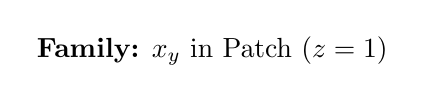
\begin{tikzpicture}
  \node[align=left] at (0,0) {\textbf{Family:} $x_y$ in Patch $(z=1)$};
\end{tikzpicture}
\end{document}
